\chapter{Metodología}

El proceso completo de clasificación puede dividirse en dos fases:

\subsubsection{Primera fase, extracción y selección de características}

\begin{figure}[H]
	\centering
	\captionsetup{justification=centering}
	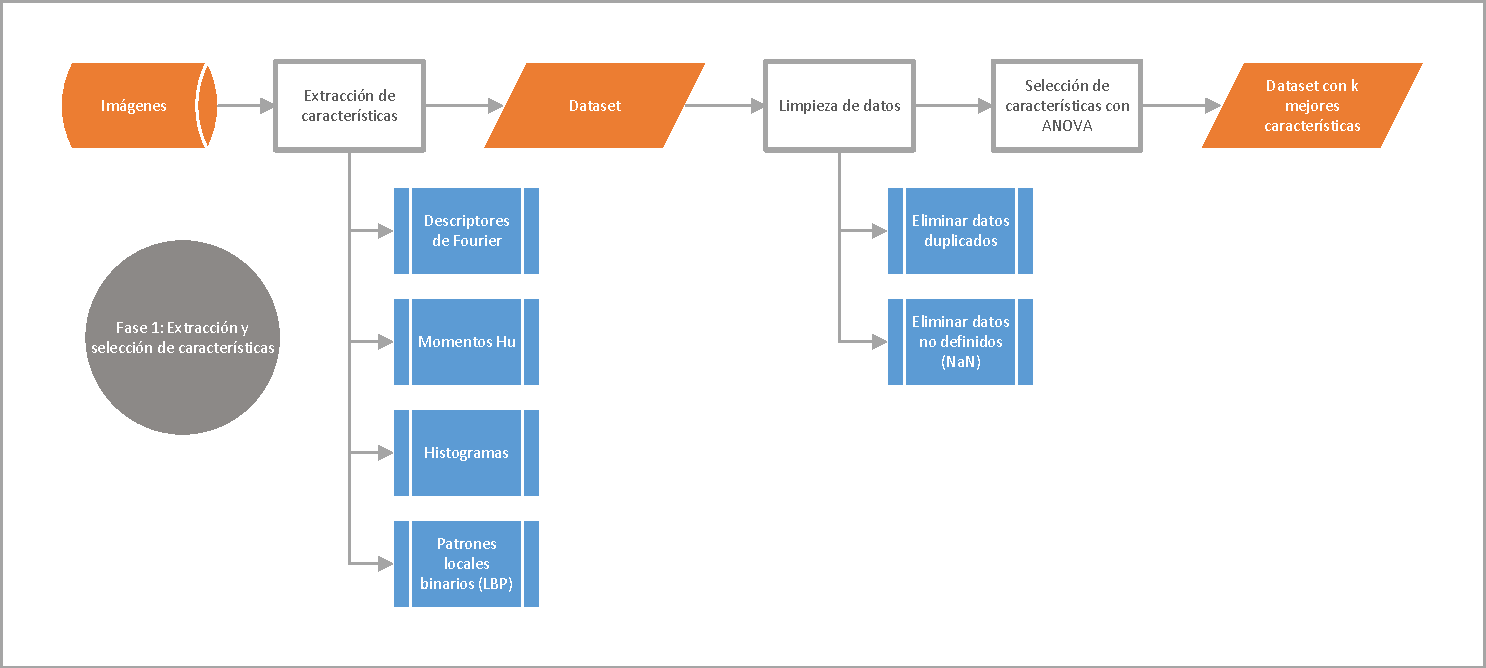
\includegraphics[width=\textwidth]{imagenes/metodología/Fase1.pdf}
	\caption{Procesos en la fase de extracción y selección de características}
	\label{met:fase1}
\end{figure}

\paragraph{Extracción de características}

El problema parte de un conjunto de imágenes almacenadas por clases y área a las que pertenecen. A partir de estas, se aplican los métodos de extracción de características. 

En el caso de extracción de Momentos Hu se ha hecho uso de la librería OpenCV, que implementa un algoritmo para extraer siete momentos Hu de una imagen binaria. 
La extracción de los histogramas de gradientes se ha realizado a partir de código propio. Los patrones locales binarios han sido implementados de igual forma con código propio. Los descriptores de Fourier han sido obtenidos haciendo uso de la librería \cite{Pybalu} para \textit{Python}, creada por Domingo Mery.

\mynote{No sé si puedo mostrarlo, pero realmente no es nada del otro mundo el código, solo unas pocas funciones no muy eficientes XD.}

De cada imagen se obtiene un vector de treinta y una posiciones (LBP ha sido descartado por no obtenerse un número uniforme de características, ya que estas dependen de la resolución de la imagen). Con un total de $n$ instancias (ó imágenes) se crea una matriz de dimensiones $nx31$, llamada $X$. Dado que los algoritmos de clasificación son supervisados, se crea, además, una matriz de etiquetas de valores $0,1,2,...,N$, siendo $N$ el número de clases, de tamaño $nx1$, llamada $Y$. Uniendo ambas matrices se obtiene el dataset.

\mynote{Normalmente un dataset se guarda como un diccionario, u objeto \textit{Bunch} de Sklearn\cite{scikit-learn}, donde sus llaves son las etiquetas, datos, datos de fourier, datos de HoG y datos de momentos, de tal forma que se puede guardar en memoria y cargarlo en cualquier momento.}

\paragraph{Limpieza de datos}

Con el dataset ya creado, es necesario entrar el proceso de limpieza de datos, que corresponde a dos subprocesos (para este caso):

\begin{itemize}
	\item Eliminación de datos duplicados: existe la posibilidad de que en el directorio de almacenamiento de imágenes exista la misma imagen duplicada varias veces, obteniéndose datos redundantes en el dataset, para ello, es necesario eliminar esos datos duplicados, dejando claro está al menos una muestra original.
	\item Eliminación de datos no definidos: En la obtención de momentos, al aplicar el escalado logarítmico es posible que algunos valores se devuelvan como indeterminados (por la naturaleza del logaritmo), de tal forma, se aplica la fórmula $Hu = -signo(Hu)log|Hu+10^{-12}|$ para obtener datos numéricos y no indeterminaciones.
\end{itemize}

\paragraph{Selección de características}

Con el dataset creado y corregido, se aplica el método de los valores F de ANOVA para obtener una descripción del poder discriminatorio de cada una de las 31 características del dataset. ANOVA se implementa a partir de la clase \textit{f\_classif} de Sklearn\cite{scikit-learn}, que devuelve un vector de tamaño $1x31$ con los 31 F valores de las características. Con la clase \textit{SelectKBest}, de Sklearn\cite{scikit-learn} también, se pueden seleccionar automáticamente, sin obtener previamente los F valores, las k mejores características en función de ANOVA.

Tras las selección de características, el dataset reduce su tamaño de $nx31$ a $nxk$.

\subsubsection{Segunda fase, selección y análisis del clasificador}

\begin{figure}[H]
	\centering
	\captionsetup{justification=centering}
	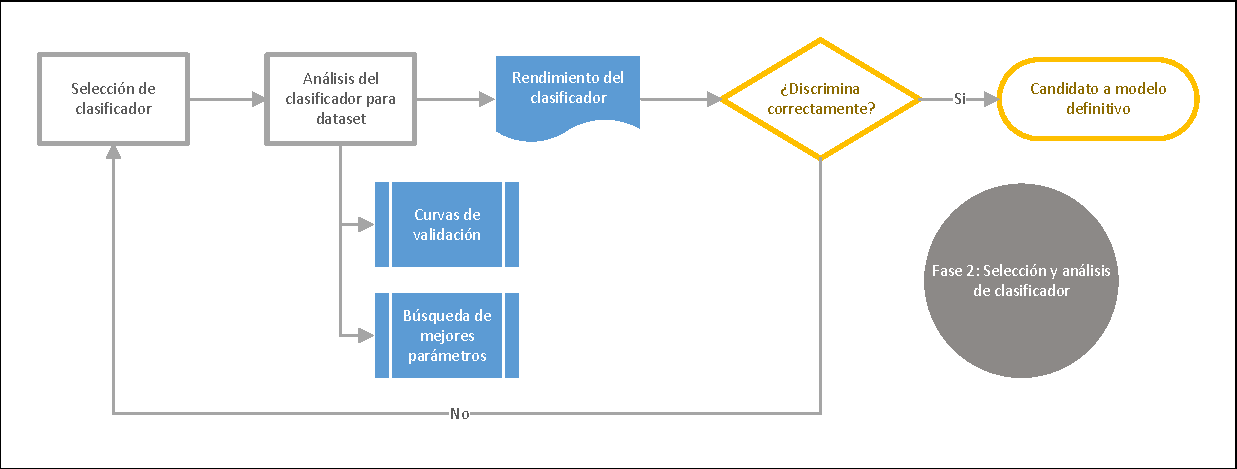
\includegraphics[width=\textwidth]{imagenes/metodología/Fase2.pdf}
	\caption{Selección y análisis del clasificador}
	\label{met:fase2}
\end{figure}

Con el dataset ya creado y las k mejores características seleccionadas se procede a realizar pruebas con diferentes clasificadores.

En primer lugar, es necesario comprobar si el dataset contiene un número balanceado de muestras, para así, poder determinar que métricas utilizar para analizar el rendimiento. 

Con un clasificador elegido para analizar su rendimiento (todos son clases de Sklearn \cite{sklearn_api}), se analiza el rendimiento del clasificador para el dataset en función de los valores de sus parámetros (curva de validación). Con este paso se consigue extraer un rango de valores para cada parámetro en el que el clasificador sobre ajuste una mínima cantidad, o discrimine perfectamente, con el cual hacer una búsqueda de los parámetros que devuelvan el mayor rendimiento para el clasificador elegido en el dataset.

Una vez obtenidos los mejores parámetros, se obtienen las métricas promedio de rendimiento (ya que es un problema multiclase) para el clasificador con esas variables. 

Si se considera que el clasificador realiza una buena discriminación, se plantea como buen candidato a modelo definitivo. De lo contrario, se escoge otro modelo de clasificador y se realiza de nuevo el mismo proceso.

%
%En este capítulo se presentan los procedimientos y técnicas empleadas para implementar y desarrollar los conceptos explicador en el capítulo \nameref{cap:marco_teorico}.
%
%El modo de funcionamiento ha consistido en implementar manualmente aquellos métodos que no pudieran obtenerse mediante librerías ya existentes. Para el resto, se ha hecho uso de las librerías de Sklearn, Numpy, OpenCV y Pybalu.
%
%\section{Implementación de los métodos de extracción de características}
%
%\paragraph{Preprocesado de imágenes} Para la tarea de lectura de imágenes, se ha hecho uso de la librería OpenCV de la siguiente forma:
%\begin{lstlisting}[language=python]	
%	img = cv2.imread(ruta+archivos)
%	img = cv2.normalize(img, 0, 255, cv2.NORM_MINMAX)    
%	gris = cv2.cvtColor(img,cv2.COLOR_BGR2GRAY)        
%	_,th = cv2.threshold(gris,0,255,cv2.THRESH_BINARY+cv2.THRESH_OTSU)	
%\end{lstlisting}
%
%La primera linea hace uso de la función \textit{imread} para leer la imagen como una matriz $\mbox{img}$. A continuación, se le aplica una normalización $\mbox{MINMAX}$, donde al mínimo valor de la imagen se le asigna el valor 0, al máximo 255, con el resto de valores siendo escalados proporcionalmente.
%
%Para los métodos que requieren imágenes binarias, las líneas 3 y 4 se utilizan para convertir la imagen de espacio RGB a escala de grises (línea 3) con la función \textit{cvtColor} y, a continuación, se implementa la función \textit{threshold} para convertir la imagen en escala de grises a binaria, según un umbral definido por un método automático (\textit{THRESH-OTSU}).
%
%Para los métodos que no requieren de una imagen binaria, las lineas 3 y 4 no son añadidas.
%
%\subsection{Momentos de imagen}
%Han sido implementados haciendo uso de la librería OpenCV (a partir de una imagen binaria):
%
%\begin{lstlisting}[language=python]	
%	momentos = cv2.moments(th)
%	hu = cv2.HuMoments(momentos)
%	for i in range(len(hu)):
%		hu[i] = -np.sign(hu[i])*np.log10(np.abs(hu[i])+1e-20)   
%\end{lstlisting}
%
%Las líneas 1 y 2 devuelven los momentos centralizados y de Hu, respectivamente. Las líneas 6 y 7 son añadidas para convertir los momentos obtenidos a una escala logarítima de más fácil comparación según la fórmula \ref{hu:escalado}. El coeficiente $1^{-20}$ es añadido para evitar que la fórmula devuelva $NaN$.
%
%\begin{equation}
%	Hu = -sgn(hu)\log\lvert Hu+1^{-20}\rvert
%	\label{hu:escalado}
%\end{equation}
%
%De esta forma presentada, para una imagen, se obtiene un vector de siete elementos con los siete momentos de Hu.
%
%\subsection{Descriptores de Fourier}
%
%Para esta tarea se ha hecho uso de la librería Pybalu\cite{Pybalu}, que implementa una función de obtención de los coeficientes de Fourier para una imagen binaria. Internamente la función está configurada para devolver los 16 primeros coeficientes. Se puede cambiar, pero véase \nameref{subsection:fourier}.
%
%\begin{lstlisting}[language=python]
%	th = (th ==255)*1
%	f = extract_features(['fourierdes'] ,bw = th)
%	f = f/np.linalg.norm(f)  
%\end{lstlisting}
%
%Al igual que con momentos, el método de los descriptores de Fourier requieren una imagen binaria. En este caso, la librería Pybalu interpreta una imagen binaria como una matriz de [0,1], por lo que requiere cambiar los valores en 255 por 1 (línea 1). La línea 2 hace una llamada a la función de extracción. La línea 3 implementa un normalizado euclidiano al vector de 16 posiciones f, para obtener un resultado comparable en todos los casos.
%
%\subsection{Histogramas de gradientes}
%
%\subsection{Patrones locales binarios}
%
%\section{Implementación de la selección de características}
%
%\subsection{SFS}
%
%El algoritmo SFS no ha sido implementado en el proceso, aún siendo un excelente método de selección de características por varias razones:
%
%\begin{itemize}
%	\item Requiere de un estimador previamente definido: SFS viene implementado como método de selección en Sklearn y Mlextend, pero ambas implementaciones requieren la definición de un modelo de clasificación previo sobre el cual basar las métricas de análisis para obtener las k mejores características. Dado que clasificadores como SVM pueden parametrizarse de muchas formas diferentes, SFS siempre devolverá un resultado diferente para cada modelo particular, por lo tanto, no se puede concluir con una selección objetiva e independiente del clasificador a seleccionar.
%	\item No devuelve los mismos resultados de la forma hacia delante frente hacia detrás.
%\end{itemize}
%
%\subsection{ANOVA}
%
%Anova, a diferencia de SFS, si devuelve información independiente del clasificador, por lo tanto, ha sido la opción elegida para la selección de características.
%
%Sklearn propociona una función para obtener los F-valores de las características de una forma muy sencilla:
%
%\begin{lstlisting}[language=python]
%	f = f_classif(X, y)
%\end{lstlisting}
%
%El método \textit{f\_classif} devuelve el vector f (F-valores) para determinar qué características escoger.
%
%\subsection{Modelos de clasificación}
%
%Para esta sección, se han utilizado por completo los clasificadores implementados en Sklearn.
%
%\subsubsection{Knn}
%
%Sklearn proporciona tanto el clasificador Knn genérico como la versión alternativa de k-centroides.
%
%\paragraph{Knn} class sklearn.neighbors.KNeighborsClassifier(n\_neighbors=k, *, weights='uniform', algorithm='auto', leaf\_size=30, p=2, metric='minkowski', metric\_params=None, n\_jobs=None)\cite{sklearn_api}
%
%\begin{itemize}
%	\item n\_neighors: nº de vecinos para determinar clasificación
%	\item weights: peso otorgado a cada muestra de entrenamiento para calcular distancias
%	\item Uniforme: todas las muestras tienen la misma influencia
%	\item Distancia: la influencia es inversa de la distancia. A mayor distancia, menos influye el punto en el resultado.
%	\item p: determina el tipo de distancia a usar (Manhattan o Euclidiana)
%	\item algorithm: sklearn determina en función del tipo de problema el mejor algortimo a usar
%\end{itemize}
%
%\paragraph{Centroide más cercano} \textit{class sklearn.neighbors.NearestCentroid(metric='euclidean')}\cite{sklearn_api}. Solo se ha de definir la distancia a usar para clasificar.
%
%\subsubsection{SVM}
%
%Sklearn proporciona tres clasificadores que siguen el planteamiento teórico de los SVM:
%
%\begin{itemize}
%	\item LinearSVC: implementación SVM de la librería liblinear que sólo permite la utilización de un kernel lineal. Está optimizado para problemas lineales y permite usar funciones de pérdida diferentes a la estándar \textit{hinge loss}.
%	\item SVC y NuSVC: implementaciones SVM de la librería libsvm. El primero utiliza el parámetro de regularización C y el segundo $\nu$.
%\end{itemize}
%
%\paragraph{LinearSVC}
%
%\section{Desarrollo}
%
%Se empieza con un directorio de carpetas de imágenes almacenadas por el área al que pertenecen en el HMI. Este conjunto de imágenes son extraídas y 
